%%%
%
% $Autor: Wings $
% $Datum: 2021-05-14 $
% $Pfad: GitLab/CornerBLending $
% $Dateiname: Hints
% $Version: 4620 $
%
% !TeX spellcheck = de_DE/GB
%
%%%



\chapter{Übersicht}

\begin{figure}[htb]
	\begin{center}
		
			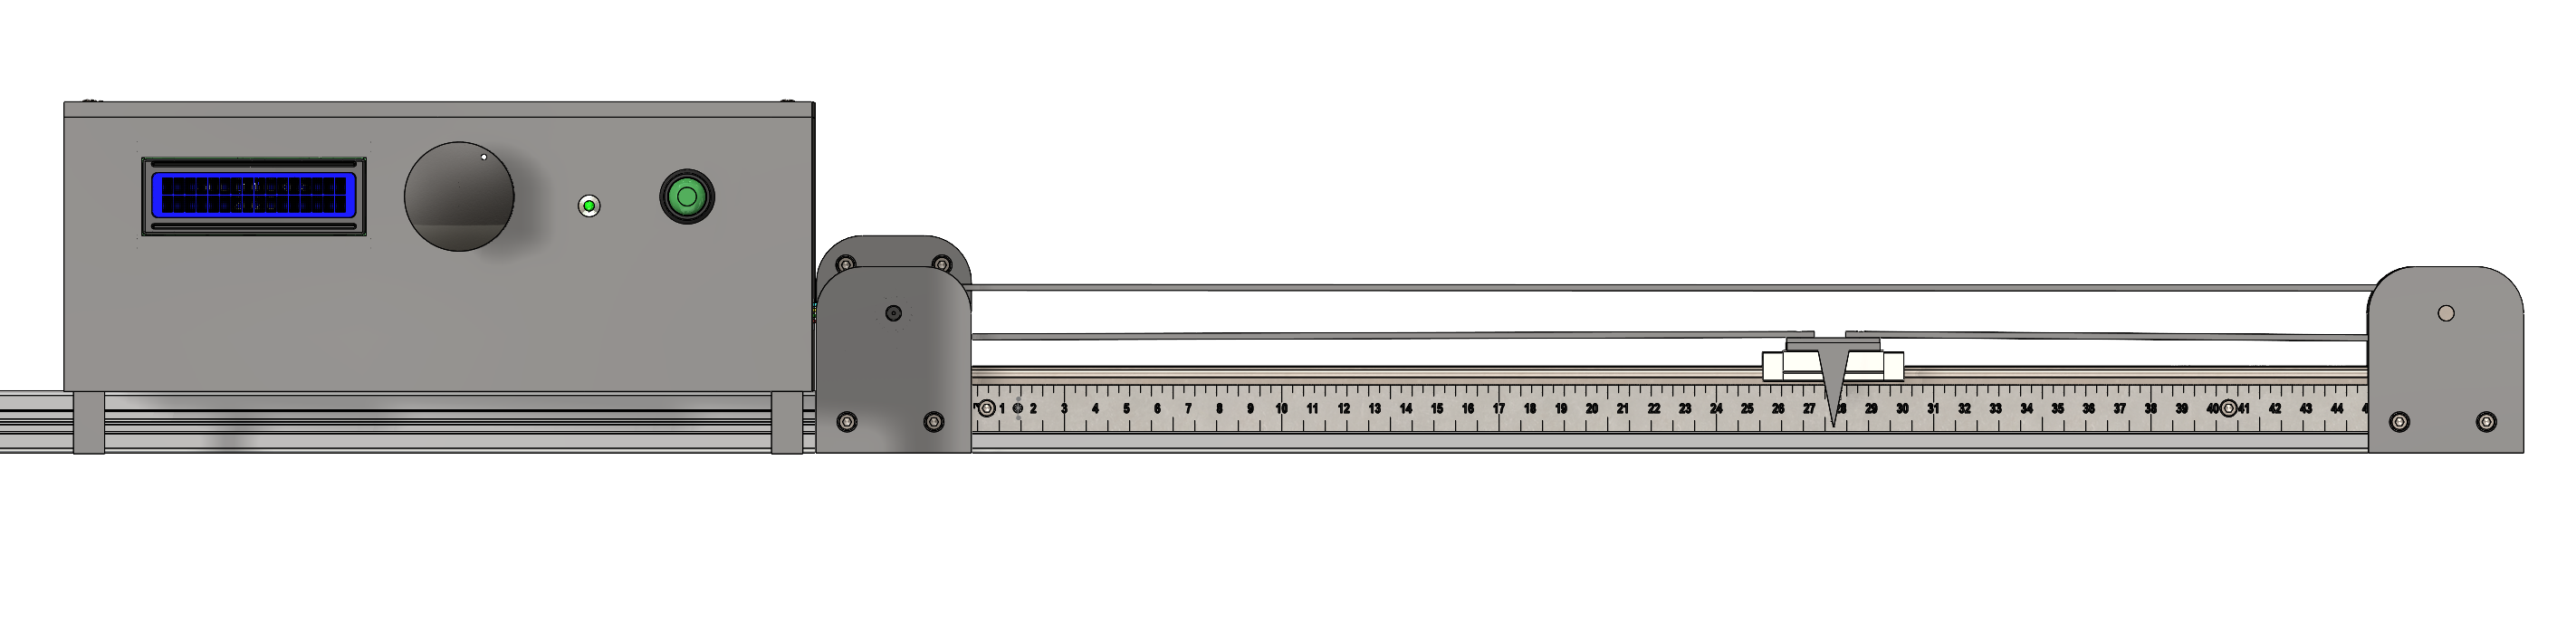
\includegraphics[width=\textwidth]{Images/Konstruktion1.png}
	%	\caption{Dies ist eine Konzeptskizze und wird noch ausgetauscht} \label{-}
	\end{center}
\end{figure}


Der Demonstrator Schrittmotor zeigt die Bewegungscharakteristik von Schrittmotoren. Mithilfe eines Anzeigepfeils werden Möglichkeiten und Grenzen von Schrittmotoren demonstriert. In zehn verschiedenen Bewegungsstufen von langsam bis schnelle Beschleunigungen verfährt der Demonstrator linear. 

\newpage
\textbf{Lieferumfang}: 
\begin{itemize}
\item Demonstrator Schrittmotor	
\item Netzkabel
	\end{itemize} 	
	\bigskip
	\textbf{Gerät aufstellen}: 
	\begin{itemize}
	\item Stellen Sie den Demonstrator auf einer ebenen, festen Oberfläche auf. Achten Sie darauf, dass das Gerät keinem direkten Sonnenlicht oder Wärme- bzw. Feuchtigkeitsquellen ausgesetzt ist. 
	\item Stellen Sie keine anderen Gegenstände auf den Demonstrator, da dies zur Fehlfunktion oder Beschädigung des Geräts führen kann. 
	\item Vergewissern Sie, dass sich keine Gegenstände im Arbeitsbereich des Demonstrators befinden.
	\end{itemize}
	\textbf{Netzanschluss}:
	\begin{itemize}
		\item Der Demonstrator wird mit einem integriertem Netzteil und \textbf{Netzkabel} ausgeliefert. Überprüfen Sie den Zustand des mitgelieferten \textbf{Netzkabel} auf Beschädigungen.
		\item Wickeln Sie das Netzkabel vom \textbf{Netzkabel-Halter}. Stecken Sie dann die Kupplung des Kabels in die Netzbuchse des Demonstrators und danach den Kontaktstecker in eine Steckdose. 
	\end{itemize} 



